\documentclass[a4paper, oneside, 12pt, openany]{book}
\pdfoutput=1

\usepackage{packages}
\addbibresource{references.bib}
\usepackage{macros}

% Prevent footnotes over multiple pages
\interfootnotelinepenalty=10000

% Label tables just like equations, theorems, definitions, etc.
%
% NB: This can be confusing if LaTeX does not place the table at the point of
% writing (e.g. for lack of space)!
\numberwithin{equation}{chapter}
\numberwithin{table}{chapter}
\makeatletter
\let\c@equation\c@table
\makeatother

% Setting up the coloured environments
%
\newbool{shade-envs}
% This can be used to toggle the coloured environments on or off.
\setboolean{shade-envs}{true}

%%
\ifthenelse{\boolean{shade-envs}}{%
  % Colours are as in Andrej Bauer's notes on realizability:
  % https://github.com/andrejbauer/notes-on-realizability
  \colorlet{ShadeOfPurple}{blue!5!white}
  \colorlet{ShadeOfYellow}{yellow!5!white}
  \colorlet{ShadeOfGreen} {green!5!white}
  \colorlet{ShadeOfBrown} {brown!10!white}
  % But we also shade proofs
  \colorlet{ShadeOfGray}  {gray!10!white}
  % For exercises
  \colorlet{ShadeOfRed}   {red!10!white}
}
% If we don't want to have shaded environments, then we use a closing symbol
% \lozenge to mark the end of remarks, definitions and examples.
{%
  \declaretheoremstyle[
      spaceabove=6pt,
      spacebelow=6pt,
      bodyfont=\normalfont,
      qed=\(\lozenge\)
  ]{definitionwithbox}
  \declaretheoremstyle[
      headfont=\itshape,
      bodyfont=\normalfont,
      qed=\(\lozenge\)
      ]{remarkwithbox}
}

% Now we set the shading using the tcolorbox package.
%
% The related thmtools' option "shaded" and the package mdframed seem to have
% issues: the former does not allow for page breaks in shaded environments and
% the latter puts double spacing between two shaded environments.
\tcbset{shadedenv/.style={
    colback={#1},
    frame hidden,
    enhanced,
    breakable,
    boxsep=0pt,
    left=2mm,
    right=2mm,
    % LaTeX thinks this is too wide (as becomes clear from the many "Overfull
    % \hbox" warnings, but optically it looks spot on.
    add to width=1.1mm,
    enlarge left by=-0.6mm}
}

% Keep a count of the number of exercises
\newtotcounter{allexercises}

\ifthenelse{\boolean{shade-envs}}{%
  \declaretheorem[sibling=equation]{theorem}
  \declaretheorem[unnumbered,title=Theorem]{theorem*}
  \declaretheorem[sibling=theorem]{lemma,proposition,corollary}
  \declaretheorem[unnumbered,title=Lemma]{lemma*}
  \declaretheorem[sibling=theorem,style=definition]{definition}
  \declaretheorem[sibling=theorem,style=definition]{example}
  \declaretheorem[sibling=theorem,style=definition]{notation}
  \declaretheorem[sibling=theorem,style=remark]{remark}
  \declaretheorem[sibling=theorem,style=definition,postheadhook=\stepcounter{allexercises}]{exercise}
  %
  \tcolorboxenvironment{theorem}    {shadedenv={ShadeOfPurple}}
  \tcolorboxenvironment{theorem*}   {shadedenv={ShadeOfPurple}}
  \tcolorboxenvironment{lemma}      {shadedenv={ShadeOfPurple}}
  \tcolorboxenvironment{lemma*}     {shadedenv={ShadeOfPurple}}
  \tcolorboxenvironment{proposition}{shadedenv={ShadeOfPurple}}
  \tcolorboxenvironment{corollary}  {shadedenv={ShadeOfPurple}}
  \tcolorboxenvironment{definition} {shadedenv={ShadeOfYellow}}
  \tcolorboxenvironment{notation} {shadedenv={ShadeOfYellow}}
  \tcolorboxenvironment{example}    {shadedenv={ShadeOfGreen}}
  \tcolorboxenvironment{remark}     {shadedenv={ShadeOfBrown}}
  \tcolorboxenvironment{proof}      {shadedenv={ShadeOfGray}}
  \tcolorboxenvironment{exercise}   {shadedenv={ShadeOfRed}}
}{% Use closing symbols if we don't have colours
  \declaretheorem[sibling=equation]{theorem}
  \declaretheorem[sibling=theorem]{lemma,proposition,corollary}
  \declaretheorem[unnumbered,title=Theorem]{theorem*}
  \declaretheorem[unnumbered,title=Lemma]{lemma*}
  \declaretheorem[sibling=theorem,style=definitionwithbox]{definition}
  \declaretheorem[sibling=theorem,style=definitionwithbox]{notation}
  \declaretheorem[sibling=theorem,style=definitionwithbox]{example}
  \declaretheorem[sibling=theorem,style=remarkwithbox]{remark}
  \declaretheorem[sibling=theorem,style=definitionwithbox,postheadhook=\stepcounter{allexercises}]{exercise}
  \tcolorboxenvironment{theorem}    {shadedenv={white}}
  \tcolorboxenvironment{theorem*}   {shadedenv={white}}
  \tcolorboxenvironment{lemma}      {shadedenv={white}}
  \tcolorboxenvironment{lemma*}     {shadedenv={white}}
  \tcolorboxenvironment{proposition}{shadedenv={white}}
  \tcolorboxenvironment{corollary}  {shadedenv={white}}
  \tcolorboxenvironment{definition} {shadedenv={white}}
  \tcolorboxenvironment{notation} {shadedenv={white}}
  \tcolorboxenvironment{example}    {shadedenv={white}}
  \tcolorboxenvironment{remark}     {shadedenv={white}}
  \tcolorboxenvironment{proof}      {shadedenv={white}}
  \tcolorboxenvironment{exercise}   {shadedenv={white}}
  }
  \declaretheorem[sibling=theorem,style=remark,numbered=no]{claim}

% Note that proofs will still have the \qed symbol at the end, even when shaded,
% because we prefer to keep up the tradition.


\begin{document}

\frontmatter

\begin{titlepage}
\begin{center}
  \vspace*{\stretch{0.5}}

  \large % Default size for the title page

  {\Huge\textsc{Categorical realizability}\par}

  \vspace{\stretch{0.2}}

  by

  \vspace{\stretch{0.2}}

  {\huge\textsc{Tom de Jong}}

  \vspace{\stretch{0.5}}

  {\Large{Lecture notes and exercises for the\\
      \textsc{Midlands Graduate School (MGS)}}} \\
  \vspace{\stretch{0.1}}
  8--12 April 2024, Leicester, UK

  \vspace{\stretch{1}}

  % \begingroup
  % \tikzset{every picture/.style={color=Gray!90!Black}}
  % \begin{tikzcd}
  %   0 & 1 & 2 & 3 & \ldots \\
  %   & & \bot \ar[ull,no head] \ar[ul,no head] \ar[u,no head] \ar[ur, no head] \ar[urr, no head]
  % \end{tikzcd}
  % \endgroup

  \begingroup
  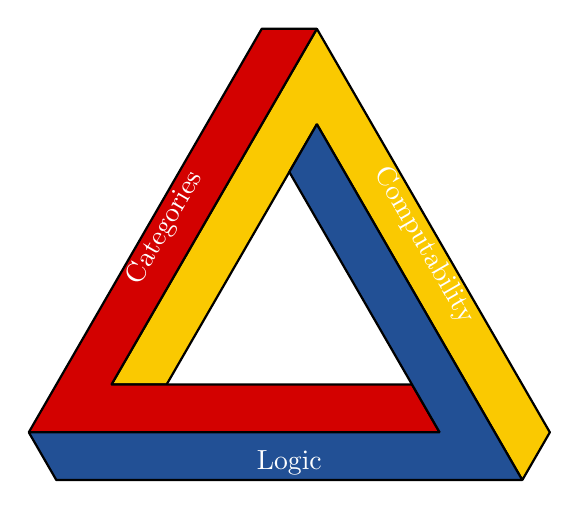
\begin{tikzpicture}[scale=1, line join=bevel]

  \definecolor{mondrianYellow}{RGB}{250,201,1}
  \definecolor{mondrianBlue}{RGB}{34,80,149}
  \definecolor{mondrianRed}{RGB}{211,1,0}

  % \a and \b are two macros defining characteristic
  % dimensions of the Penrose triangle.
  \pgfmathsetmacro{\a}{1.8}
  \pgfmathsetmacro{\b}{0.7}

  \tikzset{%
    apply style/.code     = {\tikzset{#1}},
    triangle_edges/.style = {thick,draw=black}
  }

  \foreach \theta/\facestyle/\city/\al\/\ang in {%
    %   0/{triangle_edges, fill = gray!50}/\hphantom{1pt}Computability/below/-60,
    % 120/{triangle_edges, fill = gray!25}/Categories/below/60,
    % 240/{triangle_edges, fill = gray!90}/\raisebox{5pt}{Logic}/above/0}
      0/{triangle_edges, fill = mondrianYellow}/\hphantom{1pt}Computability/below/-60,
    120/{triangle_edges, fill = mondrianRed}/Categories/below/60,
    240/{triangle_edges, fill = mondrianBlue}/\raisebox{5pt}{Logic}/above/0}
    {
    \begin{scope}[rotate=\theta]
      \draw[apply style/.expand once=\facestyle]
        ({-sqrt(3)/2*\a},{-0.5*\a})                   --
        ++  (-\b,0)                                   --
          ({0.5*\b},{\a+3*sqrt(3)/2*\b})                --node[\al=-5pt,rotate=\ang,text=White]{\city} % higher point
          ({sqrt(3)/2*\a+2.5*\b},{-.5*\a-sqrt(3)/2*\b}) -- % rightmost point
        ++({-.5*\b},-{sqrt(3)/2*\b})                    -- % lower point
          ({0.5*\b},{\a+sqrt(3)/2*\b})                  --
        cycle;
      \end{scope}
    }
   \end{tikzpicture}
  \endgroup

  \vfill

  \flushright
  {\normalsize{School of Computer Science \\
  University of Nottingham \\
  February--March 2024}}

\end{center}
\end{titlepage}

%%% Local Variables:
%%% mode: latexmk
%%% TeX-master: "../main"
%%% End:
\clearpage
\thispagestyle{empty}
\begin{flushright}
  % \vspace*{\stretch{0.5}}
  \vspace*{\fill}

  \large % Default size for the title page

  \emph{To Jaap van Oosten, \\ in recognition of
    his contributions to the teaching of
    mathematical logic.}

  \vspace*{\fill}

  \vspace{\stretch{2}}

\end{flushright}

%%% Local Variables:
%%% mode: latexmk
%%% TeX-master: "../main"
%%% End:
\restoregeometry%

\chapter{Abstract}

Realizability, as invented by Kleene, is a technique for elucidating the
computational content of mathematical proofs. In this course we study
realizability from a categorical perspective.
%
Starting from an abstract and general model of computation known as a partial
combinatory algebra (pca), we construct the category of assemblies
over it.
%
Intuitively, an assembly is a set together with computability data and an
assembly map is a function of sets that is computable. Here, the notion of
computability is prescribed by the pca.
%
Through the framework of categorical logic, the assemblies give rise to the
realizability interpretation of logic, which we spell out in detail.

The central theme of this course is the interplay between category theory, logic
and computability theory. While some familiarity with basic category theory
(e.g.\ (co)limits and adjunctions) is required for some parts of the notes, the
course hopefully offers plenty to those unfamiliar with category theory.


%%% Local Variables:
%%% mode: latexmk
%%% TeX-master: "../main"
%%% End:

\chapter{Acknowledgements}

It is my pleasure to express my sincere thanks to Jaap van Oosten---to whom I
have dedicated these notes---for teaching an excellent course on category
theory~\cite{vanOosten2016} and introducing me to realizability when I was a
master's student in mathematics at Utrecht University back in 2015--2018.

I thank Ignacio Bellas, Rahul Chhabra, Josh Chen, Stefania Damato, Johnson He,
Chris Purdy, Vincent Rahli, Alyssa Renata, Jingjie Yang and Mark Williams for
pointing out or fixing typos, and Mart\'in Escard\'o for a discussion on the BHK
interpretation.
%
I~am also grateful to Josh Chen for volunteering to be a teaching assistant for
the course.
%
For the illustration on the title page I adapted \verb|tikz| code from
\emph{AboAmmar}'s answer on \TeX\ StackExchange~\cite{latex-triangle}.

%%% Local Variables:
%%% mode: latexmk
%%% TeX-master: "../main"
%%% End:


\setcounter{tocdepth}{2}
\tableofcontents

\mainmatter%

\chapter{Introduction}

\section{Aims}

\section{Exercises}

The exercises are interspersed in the text, but each chapter ends with a list of
its exercises for reference.
%
There are \total{allexercises} exercises in total.

\section{References}

\cite{Kleene1945}
\cite{Bauer2023}\cite{vanOosten2008}
\cite{Hyland1982}\cite{HJP1980}
\cite{Bauer2006}
\cite{Streicher2018}

\section{Further reading}

\cite{Chhabra2023}
\cite{LongleyNormann2015}
\cite{Longley1995}

%%% Local Variables:
%%% mode: latexmk
%%% TeX-master: "../main"
%%% End:

\chapter[Models of computation: partial combinatory algebras]{Models of computation: \\ partial combinatory algebras}\label{chap:PCA}

The starting ingredient in categorical realizability is a general model of
computation known as a \emph{partial combinatory algebra}, or \emph{pca} for
short.
%
The desire for a general model of computation is motivated by the many possible
interesting examples.
%
Moreover, in the next chapter, we construct the \emph{category of assemblies}
over an arbitrary pca. The construction itself works generally and is
insensitive to any particular choice of pca. However, the choice of pca is
reflected in the logical principles that the resulting category validates.
%
Thinking of categories of assemblies as worlds of computable mathematics, we can
thus build different worlds by varying our notion of pca.

Having said all this, in these notes we have chosen to work with the
\emph{untyped} notion of a pca. The \emph{typed} notion, as developed by
Longley\footnote{Fun fact: John Longley is also the author of the recent
  \emph{Castles in the Air}---an introduction to the world of mathematical logic
  cast in the form of a fantasy novel---as well as a semi-professional
  pianist.} in his PhD thesis~\cite{Longley1995}, is more general and moreover
has the advantage that it can capture (idealized) typed functional programming
languages (such as PCF~\cite{Plotkin1977,deJong2023}).
%
We only treat untyped pcas for simplicity and refer the interested reader to
Bauer's more comprehensive notes~\cite{Bauer2023}.


\begin{definition}[Partial combinatory algebra (pca), \(\kcomb\), \(\scomb\)]\label{def:pca}
  A \textbf{partial combinatory algebra} (\textbf{pca}) is a set \(\AA\)
  together with a \emph{partial} operation \(\AA \times \AA \pto \AA\), denoted
  by juxtaposition, \((\pca{a},\pca{b}) \mapsto \pca{a}\pca{b}\), such that
  there exist elements \(\kcomb\) and \(\scomb\) satisfying:
  \begin{enumerate}[(i)]
  \item\label{k-behaviour} \((\kcomb \pca{a}) \pca{b} = \pca{a}\) for all elements
    \(\pca{a},\pca{b} \in \AA\),
  \item\label{s-defined} \(((\scomb \pca{f}) \pca{g})\) is defined for all elements
    \(\pca{f},\pca{g} \in \AA\), and
  \item\label{s-behaviour}
    \(((\scomb \pca{f}) \pca{g}) \pca{a} \simeq
    (\pca{f}\pca{a})(\pca{g}\pca{a})\) for all elements
    \(\pca{f},\pca{g},\pca{a} \in \AA\).
  \end{enumerate}
  The symbol \(\simeq\) is \emph{Kleene equality} and means: either both sides
  are undefined, or both are defined and are equal elements of \(\AA\).
  %
  In particular, in~\ref{k-behaviour}, the operation \(\kcomb\pca{a}\) must be
  defined for all elements \(\pca{a} \in \AA\).
\end{definition}

We think of the elements of a pca as codes for programs that can also act as
input. Accordingly, we pronounce \(\pca{a}\pca{b}\) as ``\(\pca{a}\) applied to
\(\pca{b}\)'' and think of this as: apply the program with code \(\pca{a}\) to
input \(\pca{b}\).

In this light, the element \(\kcomb\), which we call the \emph{k-combinator}, acts
as a parameterized constant program: it takes an input \(\pca{a}\) and then
always outputs \(\pca{a}\) on any input \(\pca{b}\).

The element \(\scomb\), which we call the \emph{s-combinator}\footnote{The
  letters \emph{k} and \emph{s} come from Moses Sch\"onfinkel's combinatory
  logic~\cite{Schonfinkel1924}. They respectively come from the German words
  \emph{Konstanzfunktion} (constant function) and \emph{Verschmelzungfunktion}
  (merge function). Of course, \emph{Verschmelzungsfunktion} starts with a
  \emph{v}, but Sch\"onfinkel had to avoid confusion as there was also a
  swap-arguments combinator called the \emph{Vertauschungsfunktion}.}, acts as
parameterized application: it takes two codes for programs \(\pca{f}\) and
\(\pca{g}\) and an input \(\pca{a}\) and then applies \(\pca{f}\pca{a}\) to
\(\pca{g}\pca{a}\).

\begin{notation}
  We will economize on parentheses and write \(\pca{a}\pca{b}\pca{c}\) for
  \((\pca{a}\pca{b})\pca{c}\).
  %
  We will always use the \texttt{teletype font} for arbitrary elements of a pca
  to reinforce the idea that these should be thought of as (codes of) programs.
  %
  For fixed programming constructs, we will use this \(\pcacomb{bold\; font}\)
  instead.
\end{notation}

The point of the k- and s-combinators is that they provide us with a (very
minimal) programming interface which we will explore
in~\cref{sec:basic-programming-in-pcas}.
%
We prefer to give two examples first to strengthen our intuition for pcas.

\section{Basic examples of pcas}\label{sec:basic-examples-of-pcas}

To help build some intuition for pcas, we now consider three basic examples. The
first example is a triviality, but we include it here because the category of
assemblies (see~\cref{chap:assemblies}) over it is equivalent to the familiar category of
sets.

\begin{example}[The trivial pca]
  The \textbf{trivial pca} is the singleton set \(\set{\singleton}\) with
  application map \((\singleton,\singleton) \mapsto \singleton\).
  %
  Of course, \(\kcomb \coloneq \singleton\) and \(\scomb \coloneq \singleton\).
\end{example}

\begin{example}[Untyped \(\lambda\)-calculus as a pca, \(\Lambda\)]
  Write \(\Lambda\) for the closed terms of the untyped \(\lambda\)-calculus
  quotiented by the equivalence relation generated by
  \(\beta\)-reduction. (E.g., for a closed \(\lambda\)-term \(t\), we identify
  \((\lambda{x}.{x})t\) and \(t\).)
  %
  With \(\lambda\)-calculus application the set \(\Lambda\) forms a pca with
  \(\kcomb\) and \(\scomb\) given by the equivalence classes of
  \(\lambda{xy}.x\) and \(\lambda{xyz}.(xz)(yz)\), respectively.
\end{example}

The application function of \(\Lambda\) is actually total, i.e.\ it is defined
on any two inputs. An example of a pca with a genuine partial application---which
is also the prime example of a pca---is \emph{Kleene's first model}~\cite{Kleene1945}:

\begin{example}[Kleene's first model, \(\Kone\)]\label{ex:Kleene-1}
  We define a partial application function on the set of natural numbers
  \(\Nat\): for natural numbers \(n\) and \(m\) we take \(n\,m\) to be
  \(\prenum{n}(m)\), where \(\prenum{-}\) denotes a Turing computable
  enumeration of the Turing computable partial functions on the natural numbers.

  The existence of the k- and s-combinators follows from Kleene's
  \(S^m_n\)-theorem in computability theory, see e.g.~\cite[Section~2.5.1 and
  Theorem~2.1.5]{Bauer2023} for details.

  We write \(\Kone\) for this partial combinatory algebra and return to
  it in~\cref{chap:logic}.
\end{example}

\section{Basic programming in pcas}\label{sec:basic-programming-in-pcas}

%As previously mentioned,
The k- and s-combinators of a pca provide an
interface for writing basic programs. For example, if we put\footnote{Note
  that this indeed defines an element of \(\AA\)
  by~\cref{def:pca}\ref{s-defined}.}
\(\icomb \coloneq \scomb\kcomb\kcomb\) then \(\icomb\) acts as the
identity combinator:
\(
  \icomb\pca{a} = \scomb\kcomb\kcomb\pca{a} = \kcomb\pca{a}(\kcomb\pca{a}) =
  {\pca{a}}
  \)
  for any element \(\pca{a}\) of our pca.

While theoretically possible, it is very inconvenient to program everything
directly in terms of \(\kcomb\) and \(\scomb\). Therefore, we will
define something resembling \(\lambda\)-abstraction for our pca, allowing us to
write the clearer \(\icomb \coloneq \lambdapca{x}{\var{x}}\) instead.

\begin{definition}[Terms]% over a pca]
  We fix a countably infinite set of variables, typically denoted by
  \(x,y,z,u,v,w,x_0,x_1,\dots\), and inductively define the set of
  \textbf{terms} over a pca~\(\AA\):
  \begin{enumerate}[(i)]
  \item a variable is a term,
  \item an element of \(\AA\) is a term,
  \item given two terms \(s\) and \(t\), we may form a new term denoted by \(s\,t\).
  \end{enumerate}
  A term without variables is called \textbf{closed}.
\end{definition}

\begin{notation}
  If \(t\) is a term, then we write \(t[\pca{a_1}/x_1,\dots,\pca{a_n}/x_n]\) for
  the \emph{closed} term obtained by substituting the element
  \(\pca{a_i} \in \AA\) for the variable \(x_i\) (which may or may not occur in
  \(t\)).
\end{notation}

\begin{definition}[Defined terms]
  A closed term \(r\) is \textbf{defined} if, when we interpret all subterms of
  \(r\) of the form \({s\,t}\) as \(s\) applied to \(t\) in \(\AA\), all these
  applications are defined.

  We extend this to terms with variables: such a term \(t\) is \textbf{defined}
  if for all possible substitutions of all variables in \(t\) by elements of
  \(\AA\), the resulting closed term obtained via substitution is defined.
\end{definition}

For example, the terms \(\kcomb\scomb\icomb\) and \(\scomb x\,y\) are defined.

\begin{notation}
  We extend Kleene equality from closed terms to all terms over \(\AA\): given
  two terms \(s\) and \(t\) whose variables are among \(x_1,\dots,x_n\), we
  write \(t_1 \simeq t_2\) if for all \(\pca{a_1},\dots,\pca{a_n} \in \AA\), we
  have
  \[
    t_1[\pca{a_1}/x_1,\dots,\pca{a_n}/x_n] \simeq
    t_2[\pca{a_1}/x_1,\dots,\pca{a_n}/x_n]
  \]
  as closed terms.
\end{notation}

We now define something resembling \(\lambda\)-abstraction for pcas.

\begin{definition}[``\(\lambda\)-abstraction'' in a pca, \(\lambdapca{x}{t}\)]
  For a variable \(x\) and a term \(t\), we define a new term, denoted by
  \(\lambdapca{x}{t}\), by recursion on terms:
  \begin{itemize}
  \item \(\lambdapca{x}{x} \coloneqq \icomb = \scomb\kcomb\kcomb\),
  \item \(\lambdapca{x}{y} \coloneqq \kcomb y\) if \(y\) is a variable different from \(x\),
  \item \(\lambdapca{x}{\pca{a}} \coloneqq \kcomb\pca{a}\) for \(\pca{a} \in \AA\),
  \item \(\lambdapca{x}{(t_1\,t_2)} \coloneqq \scomb(\lambdapca{x}{t_1})\,(\lambdapca{x}{t_2})\).
  \end{itemize}
\end{definition}

\begin{exercise}[Combinatory completeness]\label{exer:properties-of-lambda-pca}
  Prove that for every variable \(x\) and term~\(t\), the following properties
  of \(\lambdapca{x}{t}\) hold:
  \begin{enumerate}[(i)]
  \item The variables of \(\lambdapca{x}{t}\) are exactly those of \(t\) minus
    \(x\).
  \item\label{lambda-pca-def} The term \(\lambdapca{x}{t}\) is defined.
  \item For all \(\pca{a} \in \AA\), we have
    \((\lambdapca{x}{t})\pca{a} \simeq t[\pca{a}/x]\).
  \end{enumerate}
\end{exercise}

\begin{notation}
  We write \(\lambdapca{xy}{t}\) for the term
  \(\lambdapca{x}({\lambdapca{y}{t}})\) and similarly for more variables.
\end{notation}

Suppose we have a term \(t\) featuring only the variables \(x\), \(y\) and
\(z\), e.g., \(t \coloneqq z\kcomb x(\kcomb y)\).
%
We think of \(t\) as a \emph{partial} function
\(\AA \times \AA \times \AA \pto \AA\), taking three inputs \(\pca{a}\),
\(\pca{b}\) and \(\pca{c}\) that we may substitute in \(t\) for \(x\), \(y\) and
\(z\), respectively, and that results in the term
\(\pca{c}\kcomb\pca{a}(\kcomb\pca{b})\) which has no variables.
%
Combinatory completeness says that terms can be internalized in a pca. Indeed,
we can represent \(t\) in \(\AA\) as \(\lambdapca{xyz}{t}\). Note that this is
indeed an element of \(\AA\) by virtue
of~\cref{exer:properties-of-lambda-pca}\ref{lambda-pca-def} and the fact that
\(\lambdapca{xyz}{t}\) is a closed term.

% \begin{theorem}[Combinatory completeness]
%   For every term \(t\) with variables \(x_1,\dots,x_{n+1}\), there is an element
%   \(\pca{a} \in \AA\) such that for all
%   \(\pca{b_1},\dots,\pca{b_{n+1}} \in \AA\), we have:
%   \begin{enumerate}[(i)]
%   \item \(\pca{a}\pca{b_1}\cdots\pca{b_n}\) is defined, and
%   \item \(\pca{a}\pca{b_1}\cdots\pca{b_n}\pca{b_{n+1}}\)
%   \end{enumerate}
% \end{theorem}
% \begin{proof}
% \end{proof}

\begin{remark}
  While similar to \(\lambda\)-abstraction, we deliberately do not use the
  \(\lambda\)-symbol, because it might suggest that \(\lambdapca{x}{t}\) obeys the
  \emph{\(\beta\)-law} when substituting terms, but due to the partial nature of
  the application map, this need not be the case~\cite[p.~4]{vanOosten2008}.
\end{remark}

It is now time to make use of combinatory completeness to construct some more
combinators. We will do this in very much the same way as one encodes these
constructs in the untyped \(\lambda\)-calculus.

\subsubsection*{Booleans and conditional}\label{sec:booleans}

We define the booleans as the closed terms
\[
  \pcatrue \coloneqq \lambdapca{xy}{x} \quad\text{and}\quad \pcafalse \coloneqq
  \lambdapca{xy}{y},
\]
and the conditional as the closed term
\[
  \pcaif \coloneq \lambdapca{x}{x}.
\]
%
Note that for arbitrary \(\pca{a}\), \(\pca{b} \in \AA\), we can calculate:
\[
  \pcaif\pcatrue\pca{a}\pca{b} = \pcatrue\pca{a}\pca{b} = \pca{a}
  \quad
  \text{and}
  \quad
  \pcaif\pcafalse\pca{a}\pca{b} = \pcafalse\pca{a}\pca{b} = \pca{b}.
\]

\subsubsection*{Pairing and projection}

We define the closed terms
\[
  \pcapair \coloneqq \lambdapca{xyz}{z}{xy},
  \quad
  \pcafst \coloneqq \lambdapca{w}{w\pcatrue}
  \quad
  \text{and}
  \quad
  \pcasnd \coloneqq \lambdapca{w}{w\pcafalse}.
\]

\begin{exercise}\label{exer:pairing-projection}
  For all elements \(\pca{a}\), \(\pca{b} \in \AA\), prove that:
  \begin{enumerate}[(i)]
  \item \(\pcapair \pca{a} \pca{b}\) is defined.
  \item \(\pcafst{(\pcapair\pca{a}\pca{b})} = \pca{a}\) and
    \(\pcasnd{(\pcapair\pca{a}\pca{b})} = \pca{b}\) hold.
  \end{enumerate}
\end{exercise}

\subsubsection*{Fixed points}

We also have the fixed point combinators which are traditionally denoted by
\(\pcay\) and \(\pcaz\):
\begin{align*}
  \pcay &\coloneqq \pcaw\pcaw &\text{with}&& \pcaw &\coloneq \lambdapca{xy}{y\,(x\,x\,y)} \\
  \pcaz &\coloneqq \pcau\pcau &\text{with}&& \pcau &\coloneq \lambdapca{xyz}{y\,(x\,x\,y)\,z}
\end{align*}
These combinators satisfy:
\[
  \pcay\pca{f} \simeq \pca{f}{(\pcay\pca{f})},
    \quad
  \pcaz\pca{f} \text { is defined}
    \quad\text{and}\quad
  \pcaz\pca{f}\pca{a} \simeq \pca{f}{(\pcaz\pca{f})}\pca{a}
\]
for all elements \(\pca{f},\pca{a} \in \AA\).

\subsubsection*{Curry numerals and fundamental arithmetic}\label{sec:numerals}

For each natural number \(n \in \Nat\), we define the corresponding
\textbf{Curry numeral} \(\numeral{n}\) inductively by:
\[
  \numeral{0} \coloneq \icomb
  \quad\text{and}\quad
  \numeral{n+1} \coloneq \pcapair\pcafalse\numeral{n}.
\]

\begin{exercise}\label{exer:arithmetic}
  Define closed terms \(\pcasucc\), \(\pcapred\) and \(\pcaiszero\) such that
  for any natural number \(n \in \Nat\) the following equations hold:
  \begin{align*}
    \pcasucc\numeral{n} = \numeral{n+1},
    \quad
    \pcapred\numeral{0} = \numeral{0},
    \quad
    \pcapred\numeral{n+1} = \numeral{n}, \\
    %\quad
    \pcaiszero\numeral{0} = \pcatrue
    \quad\text{and}\quad
    \pcaiszero\numeral{n+1} = \pcafalse.
  \end{align*}

\end{exercise}

\subsubsection*{Primitive recursion}

The following \textbf{primitive recursion} combinator for Curry numerals will
come in useful when we consider the natural numbers object in the category of
assemblies later.

\begin{exercise}\label{exer:primitive-recursion}
  Construct a closed term \(\pcarec\) such that for all
  \(\pca{f},\pca{a} \in \AA\) and \(n \in \Nat\) it satisfies:
  \[
    \pcarec\pca{a}\pca{f}\numeral{0} = a
    \quad\text{and}\quad
    \pcarec\pca{a}\pca{f}\numeral{n+1} \simeq \pca{f}\numeral{n}{(\pcarec\pca{a}\pca{f}\numeral{n})}
  \]
  \emph{Hint:} The essential ingredients are a zero test, predecessor and
  repeated application which are provided by \(\pcaiszero\), \(\pcapred\) and
  \(\pcaz\), respectively.
\end{exercise}

As a final remark, we note that any nontrivial pca is necessarily infinite, as
the following exercise shows:
\begin{exercise}\label{exer:nontrivial-pca}
  Prove that the following are equivalent for any pca \(\AA\):
  \begin{enumerate}[(i)]
  \item The booleans \(\pcatrue\) and \(\pcafalse\) are distinct elements of
    \(\AA\).
  \item The Curry numerals \(\numeral{n}\) in \(\AA\) are all distinct.
    % , i.e., the map
    % \(n \in \Nat \mapsto \numeral{n} \in \AA\) is an injection.
  \item The pca \(\AA\) is not the trivial pca.
  \end{enumerate}
\end{exercise}

\section{More examples of pcas}\label{sec:more-examples-of-pcas}

In this section we will present a few more examples of partial combinatory
algebras. To motivate and introduce them, we offer the following informal
explanation. Suppose we have a device which transforms the pitch of incoming
audio. We might represent the incoming and outgoing audio as streams of bits, so
that mathematically speaking, our in- and output are elements of
\(\set{0,1}^\Nat\), i.e.\ functions from the set of natural numbers \(\Nat\) to
the two-element set \(\set{0,1}\).
%
Our bit-stream transforming device is then a function
\(\set{0,1}^\Nat \to \set{0,1}^\Nat\).
%
Since we don't want to wait forever on the output of our device, it seems
reasonable that we assume it to start outputting after having only received
finitely many bits.
%
Thus, \emph{the output depends on a finite amount of the input only}.
%
Our device should therefore not be any old function
\(\set{0,1}^\Nat \to \set{0,1}^\Nat\), but rather one whose output depends on a
finite amount of input only.
%
This can be made mathematically precise by equipping the set \(\set{0,1}^\Nat\)
with a \emph{topology} and by restricting our attention to \emph{continuous}
functions on such topologized sets.

For an introduction to and motivation of topology from a computer science
perspective, Smyth's~\cite{Smyth1992} and Escard\'o's~\cite{Escardo2004}
monographs, and Vickers's book~\cite{Vickers1996} are warmly recommended.

While Turing computable functions, or equivalently, Kleene's partial recursive
functions, provide the foundation for computability theory with (encodings of)
finite objects, an established theory of computability over infinite objects is
Weihrauch's \emph{Type Two Effectivity (TTE)}~\cite{Weihrauch2000}.
%
This is a theory of computable analysis and becomes especially relevant when we
are interested in exact real number computation.
%
Its connections to realizability were explored in the PhD theses of
Lietz~\cite{Lietz2004} and Bauer~\cite{Bauer2000} via Kleene's second model and
its recursive variant (\cref{Kleene-2,Kleene-rec-2} below).

We will be brief in our explanations of these partial combinatory algebras and hope
that the interested reader will take the above paragraphs and the examples as an
invitation to explore the fascinating connections between topology and
computability, for instance by consulting Bauer's aforementioned notes on
realizability~\cite{Bauer2023} and the references above.

Our first example is due to Scott~\cite{Scott1976} and gives the powerset of the
natural number the structure of a pca.

\begin{example}[Scott's graph model, \(\Scott\)]
  We make the powerset \(\PN\) of the natural numbers into a pca that we denote
  by \(\Scott\).

  The idea behind application on \(\PN\) is that when we apply a subset \(U\) to
  a subset \(V\), then \(U\) can only use a finite amount of \(V\) to
  determine whether to include a number or not. We now make this idea formal.

  We first fix bijections
  \[
    \pairing{{-},{-}} \colon \Nat \times \Nat \to \Nat
    \quad\quad\text{and}\quad\quad
    \enum \colon \Nat \cong \powerset_{\operatorname{fin}}(\Nat)
  \]
  where the latter enumerates all finite subsets of natural numbers.
  %
  We then define the application map \(\PN \times \PN \to \PN\) as
  \[
    (U,V) \mapsto \set{\outputnum \in \Nat \mid
            \exists(\inputnum \in \Nat) .
            \pairing{\inputnum,\outputnum} \in U \text{ and } \enum(\inputnum) \subseteq V}.
  \]
  Thus, the ``program'' \(U\) encodes a list of input-output pairs where the
  input number encodes a finite subset of the argument \(V\).

  If we equip \(\PN\) with the \emph{Scott topology} whose basic opens are
  finite subsets of \(\Nat\), then one can show that the application map is
  continuous.
  %
  In fact, any continuous function \(F : \PN^k \to \PN\) can be represented in
  \(\PN\) by encoding the graph of \(F\).
  %
  (The details are spelled out in~\cite[Example~2.3.4]{deJong2018}.)
  %
  Under this correspondence it becomes easy to construct the elements \(\kcomb\)
  and \(\scomb\) making \(\PN\) into a pca.
\end{example}

The application in the above example is actually a \emph{total} operation. An
analogous pca whose application is genuinely partial is due to
Kleene~\cite{KleeneVesley1965}:
\begin{example}[Kleene's second model, \(\Ktwo\)]\label{Kleene-2}
  Somewhat similar to the above example, we can define an application on the set
  \(\Nat^\Nat\) of functions on \(\Nat\) that makes it into a pca~\(\Ktwo\),
  known as Kleene's second model.
  %
  The encodings required for the application map are a bit involved, see
  e.g.~\cite[p.~30 and Section~2.1.2]{Bauer2023} or
  \cite[Section~1.4.3]{vanOosten2008}, but we point out that this pca is closely
  related to continuous functions \(\Nat^\Nat \to \Nat^\Nat\) where we equip
  \(\Nat^\Nat\) with the \emph{Baire topology}.
\end{example}

Another example comes from \emph{domain theory}~\cite{AmadioCurien1998} and is
also due to Scott~\cite{Scott1972}:
\begin{example}[Scott's domain model of the untyped \(\lambda\)-calculus]
  The carrier of this pca is Scott's domain \(D_\infty\) which is a model of the
  untyped \(\lambda\)-calculus via the isomorphism
  \(\Phi \colon D_\infty \simeq {D_\infty}^{D_\infty}\) of domains.
  %
  The map~\(\Phi\) sends an element \(\sigma \in D_\infty\) to a Scott
  continuous function \(\Phi(\sigma) \colon D_\infty \to D_\infty\).
  %
  We define application on \(D_\infty\) as:
  \[
    (\sigma,\tau) \mapsto \Phi(\sigma)(\tau).
  \]
\end{example}

Finally, we mention that Scott's graph model and Kleene's second model have
effective variations that are examples of \emph{elementary sub-pcas}.

\begin{definition}[Elementary sub-pca]\label{def:elementary-sub-pca}
  An \textbf{elementary sub-pca} of a pca \(\AA\) is a subset
  \(\AA^\# \subseteq \AA\) that is closed under the application of \(\AA\) and
  moreover contains the elements \(\kcomb\) and \(\scomb\) from \(\AA\).
\end{definition}

\begin{example}[Scott's r.e. graph model, \(\Scottre\)]\label{Scott-re}
  We get an elementary sub-pca \(\Scottre\) of~\(\Scott\) by restricting
  ourselves to the recursively enumerable subsets of \(\Nat\).
\end{example}

\begin{example}[Kleene's recursive second model, \(\Ktworec\)]\label{Kleene-rec-2}
  We get an elementary sub-pca \(\Ktworec\) of \(\Ktwo\) by restricting
  ourselves to the total recursive %(= Turing computable)
  functions
  \(\Nat \to \Nat\).
\end{example}

For even more examples of pcas,
see~\cite[Section~1.4]{vanOosten2008}.

\section{List of exercises}
\begin{enumerate}
\item \cref{exer:properties-of-lambda-pca}: On the fundamental properties of
  \(\lambdapca{x}{t}\).
\item \cref{exer:properties-of-lambda-pca}: On the properties of the pairing and
  projection combinators.
\item \cref{exer:arithmetic}: On fundamental arithmetic in a pca.
\item \cref{exer:primitive-recursion}: On primitive recursion in a pca.
\item \cref{exer:nontrivial-pca}: On nontriviality of a pca.
\end{enumerate}




%%% Local Variables:
%%% mode: latexmk
%%% TeX-master: "../main"
%%% End:

\chapter{Categories of assemblies}\label{chap:assemblies}


\begin{definition}[Assembly]
  An \textbf{assembly} over a pca \(\AA\) is a set \(X\) together with a
  relation \({\realizes}\) between \(\AA\) and \(X\) such that for all
  \(x \in X\), there exists at least one element \(\pca{a} \in \AA\) with
  \(\pca{a} \realizes x\).
\end{definition}

The relation \(\pca{a} \realizes x\) is pronounced as ``\(\pca{a}\)
\textbf{realizes} \(x\)'' and we also say that \(\pca{a}\) is a
\textbf{realizer} of \(x\). We think of \(\pca{a}\) as an \emph{implementation}
of \(x \in X\) in the pca.
%
The requirement on assemblies is that each element of the set must have at least
one implementation.

\begin{notation}[\(\carrier{X}\), \({\realizes_X}\)]
  Given an assembly \(X\), we will write \(\carrier{X}\) for its underlying set
  and \(\realizes_X\) for its relation between \(\AA\) and \(\carrier{X}\).
\end{notation}

\begin{example}[The assembly of booleans, \(\Two\)]
  The \textbf{assembly of booleans}, denoted by \(\Two\), is defined as
  \[
    \carrier{\Two} \coloneqq \set{0,1},
    \quad\quad
    \pcafalse \realizes_\Two 0
    \quad\quad
    \text{and}\quad\quad
    \pcatrue \realizes_\Two 1,
  \]
  where we recall the booleans \(\pcafalse\) and \(\pcatrue\) from \cref{sec:booleans}.
\end{example}

\begin{example}[The assembly of natural numbers, \(\NatAsm\)]
  The \textbf{assembly of natural numbers}, denoted by \(\NatAsm\), is defined as
  \[
    \carrier{\NatAsm} \coloneqq \Nat
    \quad\quad\text{and}\quad\quad
    \numeral{n} \realizes_\NatAsm n \text{ for each \(n \in \Nat\)},
  \]
  where we recall that \(\numeral{n}\) is the \(n\)\textsuperscript{th} Curry
  numeral from \cref{sec:numerals}.
\end{example}

\begin{example}
  Taking \(\AA = \Kone\), we can consider the assembly \(X\) of Turing computable functions:
  \[
    \carrier{X} \coloneqq \set{f \colon \Nat \to \Nat \mid f \text{ is Turing computable}}
    \quad\quad\text{and}\quad\quad
    m \realizes_X f \iff \prenum{m} = f
  \]
  where we recall \(\Kone\) and \(\prenum{-}\) from~\cref{ex:Kleene-1}.
  %
  We remark that each \(f \in \carrier{X}\) has infinitely many realizers.

  Notice that, with this realizability relation, we cannot let \(\carrier{X}\)
  be the set of \emph{all} functions from \(\Nat\) to \(\Nat\), because then the
  set of realizers of a noncomputable function would be empty, which is not
  allowed by the definition of an assembly.
\end{example}

\section{Morphisms of assemblies}

\begin{definition}[Track]
  For assemblies \(X\) and \(Y\), we say that an element \(\pca{t} \in \AA\)
  \textbf{tracks} a function \(f \colon \carrier{X} \to \carrier{Y}\) if for all
  \(x \in \carrier{X}\) and \(\pca{a} \in \AA\), if \(\pca{a} \realizes_X x\), then
  \(\pca{t}\pca{a}\) is defined and \(\pca{t}\pca{a} \realizes_Y f(x)\).
\end{definition}

\begin{notation}
  We will shorten the above to: ``\(\pca{t}\pca{a} \realizes_Y f(x)\)
  for all \(x \in \carrier{X}\) and \(\pca{a} \realizes_X x\)''.
  %
  That is, we implicitly quantify over \(\pca{a}\) and we implicitly assume that
  \(\pca{t}\pca{a}\) is defined when we write
  \(\pca{t}\pca{a} \realizes_Y f(x)\).
\end{notation}

\begin{definition}[Assembly map]
  An \textbf{assembly map} from an assembly \(X\) to \(Y\) is a function
  \(f \colon \carrier{X} \to \carrier{Y}\) that is tracked by some element.
  %
  The existence of a tracker is a required \emph{property} of the morphism and
  \emph{not} part of the data.
\end{definition}

\begin{proposition}
  Assemblies and assembly maps form a category with composition given
  by composition of functions on underlying sets.
\end{proposition}
\begin{proof}
  We need to verify that composition is well defined, i.e., that if
  \(f \colon X \to Y\) and \(g \colon Y \to Z\) are assembly maps, then
  \(g \circ f \colon \carrier{X} \to \carrier{Z}\) is tracked.
  %
  Let \(\pca{t_f}\) and \(\pca{t_g}\) track \(f\)~and~\(g\), respectively.  We
  claim that \(\lambdapca{x}{\pca{t_g}(\pca{t_f}(x))}\) tracks \(g \circ
  f\). Indeed, the closed term \(\lambdapca{x}{\pca{t_g}(\pca{t_f}(x))}\) is
  defined by construction, and if \(\pca{a} \realizes_X x\), then
  \[
    {(\lambdapca{x}{\pca{t_g}(\pca{t_f}(x)}))\pca{a} =
    \pca{t_g}(\pca{t_f}\pca{a})} \realizes_Z g(f(x))
  \]
  by choice of \(\pca{t_f}\) and \(\pca{t_g}\).
  %
  Moreover, for each assembly \(X\), we have an identity morphism on \(X\) given
  by the identity on \(\carrier{X}\) and tracked by \(\icomb\).
  %
  Finally, associativity of composition holds because composing functions of
  sets is associative.
\end{proof}

\begin{notation}[\(\Asm{\AA}\)]
  We write \(\Asm{\AA}\) for the category of assemblies over a pca \(\AA\).
\end{notation}

\begin{exercise}

\end{exercise}

\section{Categorical constructions}

\begin{exercise}\label{exer:characterise-regular-monos}

\end{exercise}

\section{Relation to the category of sets}

\begin{definition}[Forgetful functor, \(\Gamma\)]
  The \textbf{forgetful functor}
  \[
    \Gamma \colon \Asm{\AA} \to \Set
  \]
  is defined by taking an assembly \(X\) to its underlying set \(\carrier{X}\)
  and a morphism \(f \colon X \to Y\) of assemblies to the map of sets
  \(f \colon \carrier{X} \to \carrier{Y}\).
\end{definition}

\begin{exercise}\label{exer:Gamma-global-sections}
  Show that \(\Gamma\) is naturally isomorphic to the \textbf{global sections}
  functor:
  \begin{align*}
    \Asm{\AA} &\to \Set \\
    X &\mapsto \Asm{\AA}(\One,X) \\
    f \colon X \to Y &\mapsto \text{post-composition with \(f\)}
  \end{align*}
\end{exercise}

\textcolor{Mulberry}{TODO: Explain intuition for \(\nabla\). Taking an empty set
  of realizers (which is prohibited anyway) would yield a map
  \(\nabla\set{0,1} \to \Two\) which is undesirable.}
\begin{definition}[\(\nabla\)]
  We define a functor
  \[
    \nabla \colon \Set \to \Asm{\AA}
  \]
  by mapping a set \(X\) to the assembly with carrier \(X\) and
  \(\pca{a} \realizes_X x\) for \emph{any} element \(\pca{a} \in \AA\).
  %
  A map of sets \(f \colon X \to Y\) gets send to \(f\) and is tracked by
  \(\icomb\).
\end{definition}


\begin{exercise}\label{exer:Gamma-left-adjoint-to-nabla}
  Prove that \(\Gamma\) is left adjoint to \(\nabla\).
\end{exercise}

\begin{exercise}\label{exer:nabla-no-right-adjoint}
  Show that \(\nabla\) does not have a right adjoint when \(\AA\) is nontrivial.

  \emph{Hint}: Consider the assemblies \(\Two\) (recall~\cref{TODO}) and \(\nabla\set{0,1}\).
\end{exercise}

\begin{exercise}[cf.~{\cite[Lemma~5.1.7]{Zoethout2018}}]\label{exer:Gamma-no-left-adjoint}
  We assume that the pca \(\AA\) is nontrivial. The aim of these exercises is to
  conclude that \(\Gamma\) does not have a left adjoint.
  \begin{enumerate}[(i)]
  \item Show that, for any object \(X \in \Asm{\AA}\), there are at most
    \(\carrier{\AA}\)-many arrows from \(X\) to \(\Two\).
  \item Use the above to prove that the \(\AA\)-indexed coproduct of copies of
    \(\One\) does not exist in \(\Asm{\AA}\).
  \item Conclude that \(\Gamma\) does not have a left adjoint.
  \end{enumerate}
\end{exercise}

\section{List of exercises}
\begin{enumerate}
\item \cref{exer:characterise-regular-monos}: On characterising the regular
  monomorphisms.
\item \cref{exer:Gamma-global-sections}: On the forgetful functor \(\Gamma\) and
  the global sections functor.
\item \cref{exer:Gamma-global-sections}: On \(\Gamma\) being a left adjoint to
  \(\nabla\).
\item \cref{exer:nabla-no-right-adjoint}: On the non-existence of a right
  adjoint to \(\nabla\).
\item \cref{exer:Gamma-no-left-adjoint}: On the non-existence of a left
  adjoint to \(\Gamma\).
\end{enumerate}

%%% Local Variables:
%%% mode: latexmk
%%% TeX-master: "../main"
%%% End:

\chapter{The realizability interpretation of logic}\label{chap:logic}

\cite{Lawvere1969}

\begin{exercise}\label{exer:epis-monos-logically}
  Prove the following logical characterizations for any assembly map \(f \colon X \to Y\):
  \begin{enumerate}[(i)]
  \item \(f\) is a regular epimorphism if and only if
    \[
      \forall(x : X).\exists(y : Y).f(x) = y
    \]
    is realized;
  \item \(f\) is an epimorphism if and only if
    \[
      \forall(x : X).\lnot\lnot({\exists(y : Y).f(x) = y})
    \]
    is realized;
  \item \(f\) is a monomorphism if and only if
    \[
      \forall(x, x' : X).(f(x) = f(x') \Rightarrow x = x')
    \]
    is realized;
  \item \(f\) is a regular monomorphism if and only if
    \[
      \forall(y : Y).\pa*{\lnot\lnot\pa*{\exists(x : X).f(x) = y} \Rightarrow \exists!(x : X).f(x) = y}
    \]
    is realized.

    The quantifier \(\exists!\) means ``there exists a unique \dots with \dots''.

    Phrased in English, \(f\) is a regular monomorphism if and only if the statement
    \begin{quote}{``For all \(y\), if the primage of \(f\) at \(y\) is nonempty,
        then we can (effectively) find a unique \(x\) with \(f(x) = y\).''}
    \end{quote}
    is realized.
  \end{enumerate}
\end{exercise}

The \(\lnot\lnot\)-stable predicates have no computational content as made
precise by the following exercise:

\begin{exercise}\label{exer:not-not-stable-nabla-pullback}
  Show that every \(\lnot\lnot\)-stable predicate \(\phi\) on an assembly \(X\)
  is uniquely determined by a subset \(A \subseteq \carrier{X}\) such that we
  have a pullback diagram
  \[
    \begin{tikzcd}
      {[\phi]} \ar[r] \ar[d,hookrightarrow] \pbcorner
      & \nabla A \ar[d,hookrightarrow] \\
      X \ar[r,"\eta_X"] & \nabla\carrier{X}
    \end{tikzcd}
  \]
  in \(\Asm{\AA}\), where we recall that \([\phi] \hookrightarrow X\) denotes
  the mono corresponding to \(\phi\).
\end{exercise}

In fact, because subsets are uniquely determined (again, via pullback) by their
characteristic function, we have:

\begin{exercise}\label{exer:not-not-stable-nabla-two-pullback}
  Show that every \(\lnot\lnot\)-stable predicate \(\phi\) on an assembly \(X\)
  is uniquely determined by a map \(\chi \colon X \to \nabla\set{0,1}\) such
  that we have a pullback diagram
  \[
    \begin{tikzcd}
      {[\phi]} \ar[r] \ar[d,hookrightarrow] \pbcorner
      & 1 \ar[d,hookrightarrow,"{\singleton \,\mapsto\, 1}"] \\
      X \ar[r,"\chi"] & \nabla\set{0,1}
    \end{tikzcd}
  \]
  in \(\Asm{\AA}\).
\end{exercise}

The map \(1 \to \nabla\set{0,1}\) is said to be a \textbf{classifier} for the
\(\lnot\lnot\)-stable predicates (subobjects).

\section{List of exercises}
\begin{enumerate}
\item \cref{exer:epis-monos-logically}: On logical characterizations of
  (regular) epimorphisms and monomorphisms.
\item \cref{exer:not-not-stable-nabla-two-pullback}: On the correspondence
  between \(\lnot\lnot\)-stable predicates and subsets.
\item \cref{exer:not-not-stable-nabla-two-pullback}: On the classifier for
  \(\lnot\lnot\)-stable predicates.
\end{enumerate}

%%% Local Variables:
%%% mode: latexmk
%%% TeX-master: "../main"
%%% End:

\chapter{Epilogue: towards realizability toposes}\label{chap:topos}

In this epilogue we briefly discuss what is perhaps the elephant in the room (pun
intended\footnote{For the uninitiated: Johnstone's two volume compendium on
  topos theory is titled \citetitle{Elephant} and commonly referred to as ``the
  Elephant''. A third volume, covering realizability toposes was planned but has
  yet to be published.}): the \textbf{realizability topos} associated to a pca.
%
Indeed, the notion of a realizability topos is noticeably absent from these
notes, essentially because its construction is relatively complicated compared
to the category of assemblies.

Working with an (elementary) topos has some benefits of course. The primary
feature of a topos is the existence of a classifier
\(\top \colon 1 \to \Omega\) for \emph{all} monomorphisms---the category of
assemblies only has classifiers for special subclasses (e.g.\
\(\lnot\lnot\)-stable or decidable monos) as we have seen.
%
A consequence is that every monomorphism is regular (because any mono into \(X\)
is the equalizer of its characteristic map \(\chi \colon X \to \Omega\) and the
composite \(X \to \One \xrightarrow{\top} \Omega\)).
%
Thus, while regular monos and monos are distinct in the category of assemblies,
the passage to the realizability topos unifies these two concepts.

Here we briefly sketch the construction of the realizability topos over a pca.
The objects of the realizability topos are \textbf{partial equivalence
  relations}: sets \(X\) equipped with a \(\powerset(\AA)\)-valued predicate
\({\sim} : X \times X \to \powerset(\AA)\) such that transitivity and symmetry
of \(\sim\) are ``realized''.
%
For the latter we set up a Heyting prealgebra of \(\powerset(\AA)\)-valued
predicates similar to that of the realizability predicates
in~\cref{sec:cat-logic-in-asm} with the notable exception that we now work with
bare sets, so the elements of our sets are not equipped with realizers.
%
In fact, while the relation \(\sim\) is not assumed to be reflexive in
general, elements of \(x \sim x\) are taken as realizers of \(x\) and
evidence that \(x\) ``exists''.
%
In general, we think of \({\sim}\) as an equality predicate on \(X\).

A morphism between such pairs \((X,\sim_X)\) and \((Y,\sim_Y)\) is defined
to be a \(\powerset(\AA)\)\nobreakdash-valued predicate \(F\) on \(X \times Y\)
such that the statement that \(F\) is a \emph{strict} functional relation are
realized.  Strictness means
\(\forall(x\in X).\forall(y\in Y).\pa*{F(x,y) \Rightarrow x \sim_X x \land y
  \sim_Y y}\), that is, \(F\) relates only elements that ``exist''.
%
Moreover, \(F\) should respect the equality predicates, i.e.\
\(\forall(x,x'\in X).\forall(y,y' \in Y).\pa*{F(x,y)\land(x\sim_X
  x')\land(y\sim_Y y') \Rightarrow F(x',y')}\) must be realized.
%
Finally, \(F\) should be a \emph{functional} relation, so we also require
single-valuedness and totality, in the sense that
\(\forall(x\in X).\forall(y,y' \in Y).\pa*{F(x,y) \land F(x,y') \to y \sim_Y
  y'}\) and \(\forall(x \in X).(x \sim_X x \to \exists(y \in Y).F(x,y))\) are
realized.

One can show that the resulting category is indeed a topos and that it houses
the category of assemblies as a full subcategory. In fact, the category of
assemblies is precisely the subcategory of \(\lnot\lnot\)-separated objects of
the realizability topos, i.e.\ those objects \(X\) for which
\(\forall(x,y:X).(\lnot\lnot(x=y) \to (x=y))\) holds in the internal logic.
%
This is perhaps foreseen by the ``classical'' interpretation of equality in the
realizability logic of assemblies (\cref{realizability-logic}).

The realizability topos over Kleene's first model is known as \textbf{the
  effective topos} as was detailed in Hyland's landmark paper~\cite{Hyland1982}.
%
The more general theory, known as \textbf{tripos theory}, was the subject of
Pitts's PhD thesis~\cite{Pitts1981} and his joint paper with Hyland and
Johnstone~\cite{HJP1980}.
%
The interested reader can consult van Oosten's textbook~\cite{vanOosten2008},
Streicher's notes~\cite{Streicher2018}, or Zoethout's master's
thesis~\cite{Zoethout2018}.

%%% Local Variables:
%%% mode: latexmk
%%% TeX-master: "../main"
%%% End:


\backmatter%
\printbibliography[heading=bibintoc]%

\end{document}
